% !TEX root = ./thesis.tex

\chapter{Evaluation}
\label{cha:eval}

\section{Evaluation dataset}
\subsection{Data collection}

Access to large ammount of training data is crucial for appying deep learning models.
Successes of deep learning on image recognition and segmentation tasks can be attributed to existance of large research datasets as ILSVRC and Places365 \cite{ILSVRC15, Zhou2016} containing millions of labeled images.
Machine translation, NLP tasks \cite{Karpathy2014, Kim2014} often rely on low-dimensional word embedding models.
Such models, as for example as word2vec or Glove \cite{Mikolov2013, pennington2014glove}, are trained on terabytes of textual data.
Deep reinforcement models might use existing gaming engines to generate required training data "on the go".
As, for example Google DeepMind team uses Atari 2D games to generate data for Q-learning \cite{Mnih2013}.

For the purpose of this research we collect visual data using ViZDoom AI research platform \cite{Kempka2016}.
ViZDoom is a Doom-based platform for reinforcement learning.
It provides access to raw visual data from Doom gaming engine.
Doom is a first-person shooter (FPS) computer game utilizing 3D graphics.
In context of our research ViZDoom platform allows automatic visual data generation and collection.

We created multiple Doom maps specifically for our task using Slade \cite{Slade3} software.
Created maps provide high diversity of textures for better discrimination between images, captured from different positions on the map.
Other reason for diverse structures on the map is to explicitly brake simmetry of the map.
Symmetric maps look alike from different player positions.
Such position tend to be encoded with the same values of sparce features.
This represents a difficulty for evaluation and comparison of quality of sparce features.

We record multiple movement trajectories on each map.
More specifically, we record 10000-60000 consequtive images of unstructured movement of the player on the map for training purposes.
In addition to that, we record movement along well defined structured trajectories as a "circle" or an "eight" for model evaluation and comparison of quality of extracted features.


\begin{figure}
\centering
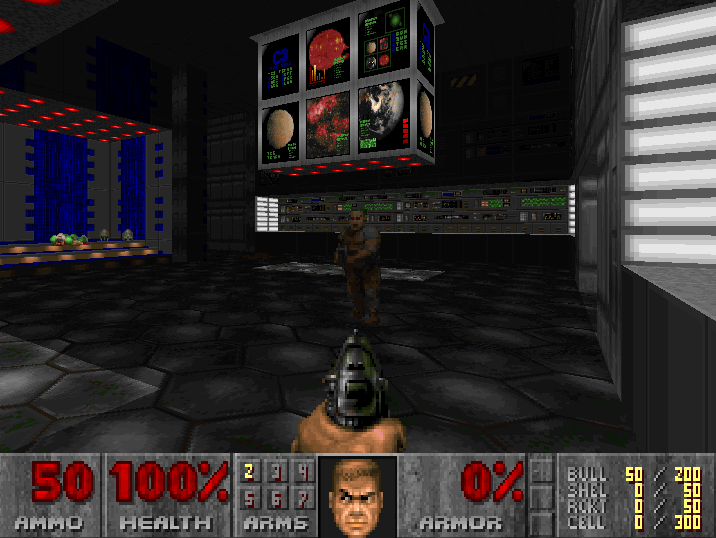
\includegraphics[width=.80\textwidth]{doom.png} %{CS0031}
\caption{Example of DoomII image collected with ViZDoom \cite{Kempka2016}.}
\label{fig:doom}
\end{figure}

\subsection{Dataset description}

Say few words about how your datasets look like and what trajectories you follow

\subsection{Data format}

Tell what is on the pictures
